\section{Thuật toán Tiến hóa Đa yếu tố (MFEA)} % (fold)
\label{sec:Thuật toán Tiến hóa Đa yếu tố (MFEA)}

\subsection{Việc phân loài trong MFEA} % (fold)
\label{sub:Việc phân loài trong MFEA}

\begin{frame}{Việc phân loài trong MFEA}
  Lấy ý tưởng từ các loài trong tự nhiên, thuật toán MFEA chia quần thể hiện tại
  thành các loài ứng với các bài toán. Một cách tự nhiên, ta có thể coi một cá thể \( p
  \) là cá thể loài \( i \) (\( i \in \{1, 2, \ldots , T\}   \)) nếu nó "phù hợp
  nhất" đối với bài toán \( i \).

  Ta cần chỉ rõ rằng một cá thể như thế nào là "phù hợp nhất"
  với một bài toán. Chẳng hạn, ta có thể sử dụng trực tiếp hàm fitness:
  \[
    i = \operatorname*{argmin}_{1 \le j \le  T} \{f_{j}(x)\}  \iff x \text{ "phù
    hợp nhất" với bài toán thứ } i
  .\] 
  Tuy nhiên, việc so sánh trực tiếp các hàm fitness không nên được dùng, do các
  hàm fitness của các bài toán khác nhau có các miền giá trị khác nhau. Do đó,
  ta sử dụng một giá trị có miền giá trị cố định hơn: thứ tự của cá thể trong
  quần thể khi sắp xếp theo thứ tự giảm dần của hàm fitness của bài toán thứ \(
  i\), hay \textbf{factorial rank} của cá thể đối với bài toán thứ \( i \):
  \[
    i = \operatorname*{argmin}_{1 \le j \le  T} \{r_{j}(x)\}  \iff x \text{ "phù
    hợp nhất" với bài toán thứ } i
  .\] 
\end{frame}

\begin{frame}{Việc phân loài trong MFEA}
  Khi xác định factorial rank, các cá thể có cùng giá trị fitness đối với bài
  toán thứ \( j \), gọi là \textbf{\( j \)-counterparts}, sẽ được sắp xếp ngẫu nhiên và
  có factorial rank khác nhau. Nếu các \( j \)-counterparts là cùng loài, chúng
  được gọi là \textbf{strong counterparts}.

  "Loài" trong MFEA được mô phỏng bởi \textbf{skill factor}. Skill factor của cá
  thể \( x \) được ký hiệu là \( \tau (x) \):
  \begin{align*}
    \tau (x) = i &\iff x \text{ "phù hợp nhất" với bài toán thứ } i\\
                 &\iff i = \operatorname*{argmin}_{1 \le j \le  T} \{r_{j}(x)\} 
  .\end{align*}

  Khi MFEA sử dụng thêm hàm phạt để hạn chế các cá thể vi phạm ràng buộc, giá
  trị của hàm fitness sau khi cộng thêm hàm phạt của một cá thể được gọi là
  \textbf{factorial cost}. Ở đây, ta coi như việc cộng thêm hàm phạt thuộc về
  từng bài toán, nên factorial cost và fitness coi như là một.
\end{frame}

\begin{frame}{Việc phân loài trong MFEA}
  Trong MFEA, mỗi cá thể có \( T \) giá trị fitness ứng với \( T \) bài toán. Để
  so sánh giữa các cá thể khác loài trong MFEA, người ta đưa ra một giá trị
  fitness chung mọi bài toán, gọi là \textbf{scalar fitness}:
  \[
    \varphi(x) = \frac{1}{\min\limits_{1 \le j \le  T} r_{j}(x)}=
    \frac{1}{r_{\tau (x)}(x)}
  .\] 
  Sử dụng scalar fitness ta có thể so sánh giữa các cá thể. Cá thể \( x \) gọi
  là \textbf{trội hơn} cá thể \( y \) nếu như nó có scalar fitness lớn hơn: \( x
  \gg y \iff \varphi(x) > \varphi(y) \).
\end{frame}

\begin{frame}{Việc phân loài trong MFEA}
  \[
    \begin{array}{c| c c c c}
      
    \end{array}
  .\] 
\end{frame}
% subsection Việc phân loài trong MFEA (end)

\subsection{Thuật toán chung của MFEA} % (fold)
\label{sub:Thuật toán chung của MFEA}

\begin{frame}[fragile]
\frametitle{Thuật toán chung của MFEA}
Về cấu trúc chung, thuật toán MFEA có dạng giống như một thuật toán tiến hóa cơ
bản. Điểm khác biệt lớn nhất là sau khi sinh ra các cá thể mới, các giá trị
skill factor và scalar fitness của mọi cá thể cần được cập nhật (hàm
$\texttt{update\_mfea\_values}$):
\begin{minted}[fontsize=\small]{python}
def mfea():
  population = init_pop()
  update_mfea_values(population)

  while True:
    reproduction(population)
    update_mfea_values(population)
    selection(population)
    yield population
\end{minted}
\end{frame}

\begin{frame}[fragile]
\frametitle{Thuật toán chung của MFEA}
Do skill factor và scalar fitness phụ thuộc vào factorial rank, nên các giá trị
này phụ thuộc vào cả quần thể chứ không phải chỉ một mình cá thể. Do đó, khi cập
nhật các giá trị này, ta cần tiến hành cập nhật với mọi cá thể trong quần thể:
\begin{minted}[fontsize=\footnotesize]{python}
def update_mfea_values(population):
  # Tính factorial rank
  for task in tasks:
    # Sắp xếp quần thể theo factorial cost (fitness)
    population.sort(key=lambda x: x.factorial_cost[task], reverse=True)
    for i, x in enumerate(population): # lặp cùng chỉ số
      x.factorial_rank[task] = i + 1 # cộng 1 do chỉ số bắt đầu từ số 0

  # Từ factorial rank tính skill factor và scalar fitness
  for x in population:
    # skill factor là bài toán mà x có factorial rank thấp nhất
    x.skill_factor = min(tasks, lambda task: x.factorial_rank[task])
    # scalar fitness tính thông qua skill factor
    x.scalar_fitness = 1 / x.factorial_rank[x.skill_factor]
\end{minted}
\end{frame}

\begin{frame}[fragile]
\frametitle{Thuật toán chung của MFEA}
\begin{minted}[fontsize=\small]{python}
def mfea():
  population = init_pop()
  update_mfea_values(population)

  while True:
    reproduction(population)
    update_mfea_values(population)
    selection(population)
    yield population
\end{minted}

Sử dụng scalar fitness, ta có thể tiến hành chọn lọc trong MFEA sử dụng các toán
tử chọn lọc như trong giải thuật di truyền. Đây cũng là lý do vì sao ta thực
hiện bước chọn lọc sau khi tính toán hết các scalar fitness và skill factor.
\end{frame}

% subsection Thuật toán chung của MFEA (end)

\subsection{Toán tử sinh sản trong MFEA} % (fold)
\label{sub:Toán tử sinh sản trong MFEA}

\begin{frame}[fragile]
\frametitle{Toán tử sinh sản trong MFEA}
MFEA lấy ý tưởng từ hai hiện tượng xảy ra trong tự nhiên và xã hội:
\begin{itemize}
\item Giao phối chọn lọc (Assortative Mating): các cá thể trong tự nhiên có xu
  hướng giao phối với các cá thể có các đặc điểm giống cá thể này. Ở đây, các cá
  thể sẽ ưu tiên giao phối cùng loài:
\begin{minted}[fontsize=\small]{python}
import random

def reproduction(population):
  for p1, p2 in pick_mating_parents(population):
    # nếu không cùng loài, chỉ thực hiện giao phối với xác suất `rmp`
    if p1.skill_factor == p2.skill_factor or random.random() < rmp:
      create_offspring(population, p1, p2) # tạo con và thêm vào quần thể
    else:
      create_mutant(population, p1) # tạo con là các đột biến của
      create_mutant(population, p2) # hai cá thể cha mẹ
\end{minted}
Ở đây, tham số $\texttt{rmp}$ (random mating probability) điều chỉnh xác suất
lai ghép khác loài.
\end{itemize}
\end{frame}

\begin{frame}[fragile]
\frametitle{Toán tử sinh sản trong MFEA}
MFEA lấy ý tưởng từ hai hiện tượng xảy ra trong tự nhiên và xã hội:
\begin{itemize}
\item Chuyển giao văn hoá dọc (Vertical Cultural Tranmission): Chuyển giao văn
  hóa có hai loại: ngang (từ các cá thể cùng thế hệ) và dọc (từ các cá thể cha
  mẹ, tổ tiên). MFEA chỉ sử dụng chuyển giao văn hóa dọc.
\end{itemize}
  \begin{figure}
    \centering
    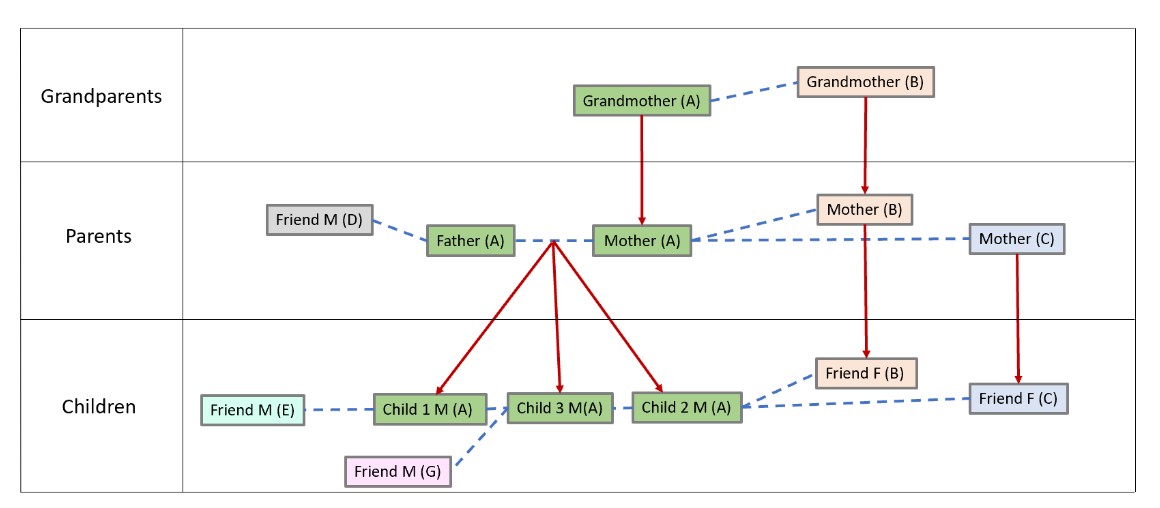
\includegraphics[height=0.5\textheight]{res/vct.png}
    \caption{Mạng các mối quan hệ của một người trong một nhóm nhỏ.}
  \end{figure}
\end{frame}

\begin{frame}[fragile]
\frametitle{Toán tử sinh sản trong MFEA}
Trong MFEA, văn hóa được chuyển giao chính là thông tin về loài. Cá thể con sẽ
kế thừa skill factor từ cá thể cha mẹ của nó:
\begin{minted}[fontsize=\footnotesize]{python}
def create_offspring(population, p1, p2):
  for c in crossover(p1, p2): # thực hiện lai ghép (có thể sinh ra nhiều con)
    # ép cá thể con phải có skill factor của một trong hai cá thể cha mẹ
    c.skill_factor = random.choice([p1.skill_factor, p2.skill_factor])
    c.factorial_cost[c.skill_factor] = fitness(c.skill_factor, c)
    population += [c]

def create_mutant(population, p): # thực hiện đột biến, tương tự như trên
  c = mutate(p)
  c.skill_factor = p.skill_factor
  c.factorial_cost[c.skill_factor] = fitness(c.skill_factor, c)
  population += [c]
\end{minted}

Khi skill factor của cá thể con được cập nhật, thì do các factorial cost của nó
đối với các bài toán khác bài toán skill factor bằng \( +\infty \), nên skill
factor của nó không đổi.
\end{frame}

% subsection Toán tử sinh sản trong MFEA (end)

\subsection{Tổng quát hóa thuật toán MFEA} % (fold)
\label{sub:Tổng quát hóa thuật toán MFEA}

\begin{frame}{Decision Variable Translation Strategy}
  Xét bài toán tối ưu đa nhiệm sau:
  \begin{align*}
    f_{1}(x) &= (x_{1}-1)^2+(x_{2}-2)^2 \\
    f_{2}(x) &=  (x_{1}+1)^2+(x_{2}+2)^2 \\
    X_{1} &= X_{2} = \mathbb{R}^2
  .\end{align*}
  Thì khi thuật toán hội tụ, các cá thể hai loài sẽ nằm lần lượt trong hai lân cận \(
  [1-\varepsilon,1+\varepsilon] \times [2-\varepsilon, 2+\varepsilon] \) và \(
  [-1-\varepsilon, -1+\varepsilon] \times [-2-\varepsilon, -2+\varepsilon] \).
  Nếu ta sử dụng các phép lai ghép như N-point Crossover hay SBX, một cá thể
  được lai từ hai loài sẽ luôn kém tối ưu hơn cha mẹ nó, nên việc chuyển giao
  tri thức không còn hiệu quả.

  Mặt khác, ta dễ thấy rằng hai hàm mục tiêu có biểu hiện trên giống y hệt nhau
  ở gần điểm cực tiểu \( (1, 2) \) và \( (-1, -2) \), nên rõ ràng vẫn có thông
  tin có thể chuyển giao giữa hai bài toán.
\end{frame}

\begin{frame}[fragile]
\frametitle{Decision Variable Translation Strategy}
  Để khắc phục vấn đề này, trước khi lai ghép, ta có thể thực hiện một bước
  \textbf{tịnh tiến} các cá thể cha mẹ lại gần nhau, sau đó thực hiện lai ghép
  và tịnh tiến ngược lại cá thể con tùy theo skill factor của cá thể này:
% https://q.uiver.app/#q=WzAsOCxbMCwwLCJwXzEiXSxbMCwyLCJwXzIiXSxbMiwwLCJwXzEnIl0sWzIsMiwicF8yJyJdLFs0LDAsImNfMSciXSxbNCwyLCJjJ18yIl0sWzYsMCwiY18xIl0sWzYsMiwiY18yIl0sWzAsMiwiVF8xIl0sWzEsMywiVF8yIiwyXSxbMyw0XSxbMiw1XSxbMiw0LCJcXHRleHR7bWF0aW5nfSJdLFszLDUsIlxcdGV4dHttYXRpbmd9IiwyXSxbNCw2LCJUXzFeey0xfSJdLFs1LDcsIlRfMl57LTF9IiwyXV0=
\[\begin{tikzcd}[cramped]
	{p_1} && {p_1'} && {c_1'} && {c_1} \\
	\\
	{p_2} && {p_2'} && {c'_2} && {c_2}
	\arrow["{T_1}", from=1-1, to=1-3]
	\arrow["{T_2}"', from=3-1, to=3-3]
	\arrow[from=3-3, to=1-5]
	\arrow[from=1-3, to=3-5]
	\arrow["{\text{mating}}", from=1-3, to=1-5]
	\arrow["{\text{mating}}"', from=3-3, to=3-5]
	\arrow["{T_1^{-1}}", from=1-5, to=1-7]
	\arrow["{T_2^{-1}}"', from=3-5, to=3-7]
\end{tikzcd}\]

Ở ví dụ trên, các cá thể cha mẹ được tịnh tiến trước khi thực hiện lai ghép,
sinh ra hai con có hai skill factor khác nhau. Hai cá thể con này sẽ được tịnh
tiến ngược lại để được thêm vào quần thể.
\end{frame}

\begin{frame}[fragile]
\frametitle{Decision Variable Translation Strategy}
Để xác định các phép tịnh tiến \( T_{i} \) cho bài toán thứ \( i \), một sự lựa
chọn tự nhiên là phép tịnh tiến thỏa mãn điều kiện sau:
\[
  T_{i}(m_{i}) = cp \implies T_{i}(x) = x + (cp - m_{i})
.\]
Trong đó, điểm \( cp \) (chẳng hạn \( cp = (0.5, 0.5, \ldots , 0.5) \)) là một
vị trí cố định trong không gian chung. \( m_{i} \) là một vector đại diện cho
các vector có loài thứ \( i \) (skill factor bằng \( i \)).

Ta có thể lấy \( m_{i} \) là vector trung bình của top \( \mu \% \) các cá thể
có loài thứ \( i \):
\begin{gather*}
  m_{i} =  \frac{1}{\mu N_{i}}\sum_{\substack{x \in P\\\tau (x) = i\\ r_{i}(x)
  \le \mu N_{i}}}(x), i=\overline{1,T}
\end{gather*}
\( N_{i} \) ở đây là số cá thể có skill factor là \( i \) trong quần thể.
\end{frame}

\begin{frame}[fragile]
\frametitle{Decision Variable Translation Strategy}
Vector tịnh tiến còn được nhân thêm với hai tham số để tối ưu việc tịnh tiến:
\begin{itemize}
\item \( sf \) (scale factor): Khi các cá thể đang hội tụ đến một điểm, vector
  \( m_{i} \) có thể chưa phản ánh đúng vị trí cực tiểu thực sự, nên vector \(
  cp-m_{i} \) có thể có sự sai lệch nhỏ. \( sf \) được nhân thêm nhằm chỉnh lại
  sai số này.

\item \( \alpha \): Do \( m_{i} \) càng ngày càng tiến đến chính xác hơn vị trí
  tối ưu, nên ta sẽ cho tham số này tăng dần trong quá trình chạy thuật toán như
  sau:
  \[
    \alpha = \left( \frac{g}{G} \right) ^2
  .\]

  Trong đó, \( g \) và \( G \) lần lượt là số thế hệ hiện tại và số thế hệ tối
  đa.
\end{itemize}
\[
  T_{i}(x) = x + sf \cdot \alpha(cp - m_{i})
.\] 
\end{frame}

\begin{frame}[fragile]
\frametitle{Decision Variable Translation Strategy}
Ngoài ra, việc liên tục cập nhật các phép tịnh tiến này sẽ làm cho thuật toán
chạy không ổn định và không thể hội tụ. Vì thế nên ta sẽ chỉ cập nhật các \(
T_{i} \) khoảng \( \theta \) thế hệ một lần.

Mặt khác, do các giá trị \( m_{i} \) không phản ánh chính xác vị trí tối ưu trong
những thế hệ đầu, nên ta sẽ chỉ bắt đầu cập nhật các \( T_{i} \) sau \( \phi \)
thế hệ.

\begin{minted}{python}
def try_update_translations(generation):
  if generation > phi and generation % theta == 0:
    update_translations(generation)
\end{minted}

Cách thực hiện tịnh tiến và cập nhật vector tịnh tiến trên được gọi là
\textbf{Decision Variable Translation Strategy} (DVTS).
\end{frame}

\begin{frame}[fragile]
\frametitle{Decision Variable Shuffling Strategy}
Tiếp tục xét bài toán sau:
\begin{align*}
  f_{1}(x) &= x_{1}^2+x_{2}^2 \\
  f_{2}(x) &= \operatorname{Ackley}(x) \\
  X_{1} &= \mathbb{R}^2, X_{2} = \mathbb{R}^{100}
.\end{align*}
Hàm \( f_{2} \) là hàm Ackley 100 chiều, một hàm số hay được sử dụng trong thử
nghiệm các thuật toán tối ưu. Hàm này có nhiều nghiệm tối ưu địa phương nên
tương đối khó tối ưu.
\begin{figure}
  \centering
  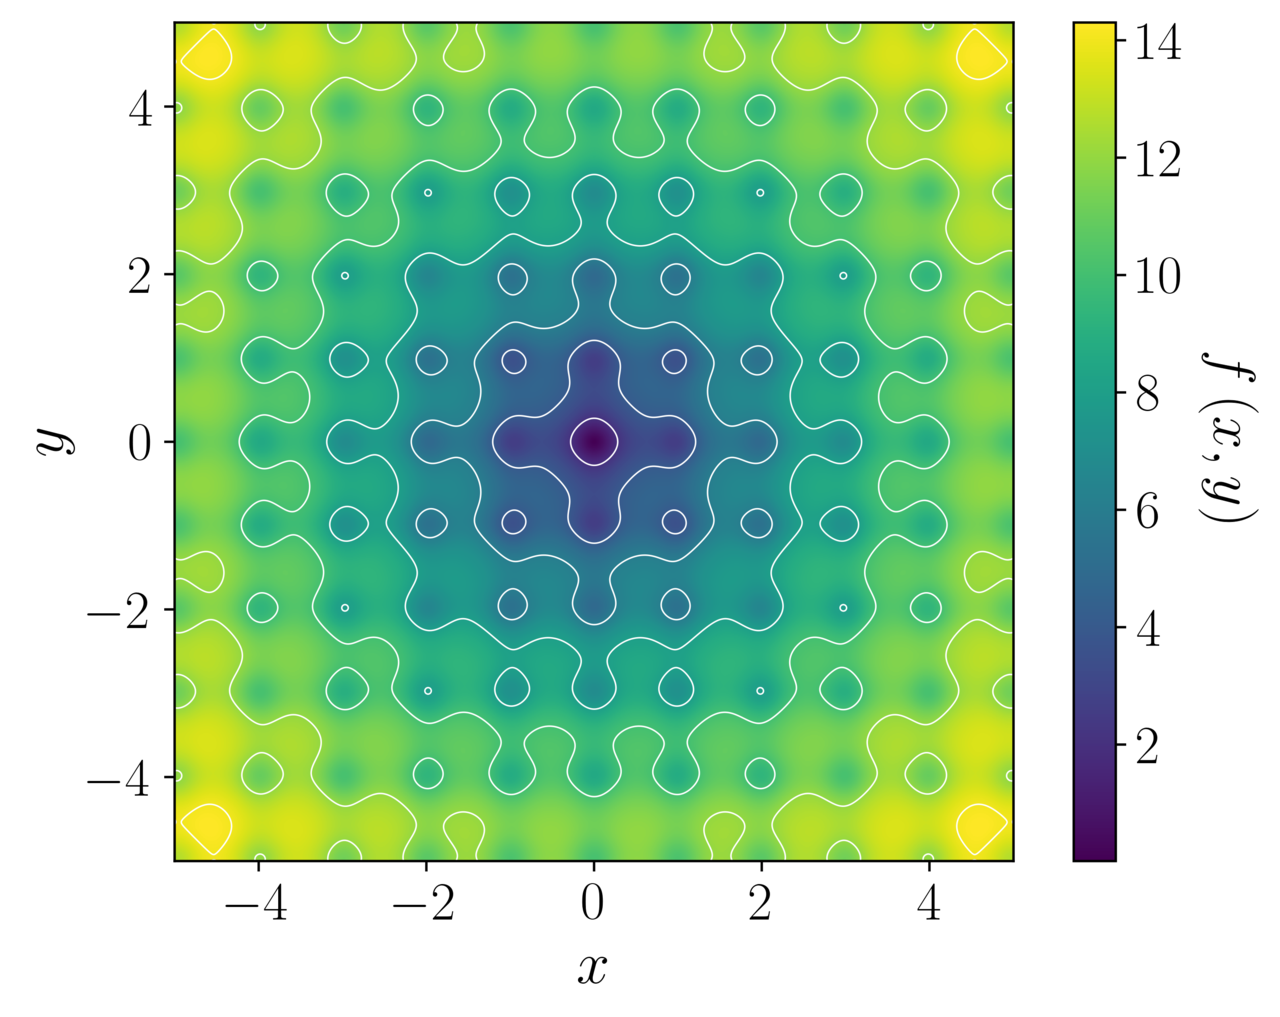
\includegraphics[height=0.3\textheight]{res/ackley.png}
  \caption{Đồ thị màu hàm Ackley trong hai chiều.}
\end{figure}
\end{frame}

\begin{frame}[fragile]
\frametitle{Decision Variable Shuffling Strategy}
\begin{align*}
  f_{1}(x) &= x_{1}^2+x_{2}^2 \\
  f_{2}(x) &= \operatorname{Ackley}(x) \\
  X_{1} &= \mathbb{R}^2, X_{2} = \mathbb{R}^{100}
.\end{align*}
Hai hàm số có cực tiểu giống nhau (đều là vector không), nên ta sẽ mong muốn
MFEA sử dụng tính tương đồng này để chuyển giao tri thức từ hàm dễ tối ưu hơn
(hàm \( f_{1} \)) sang hàm khó tối ưu hơn (hàm \( f_{2} \)).

Tuy nhiên, thuật toán hiện tại của ta chỉ có thể chuyển giao được tri thức của
hai gen đầu, vì số chiều của bài toán thứ nhất chỉ bằng 2. Nếu lựa chọn phép đột
biến phù hợp, thì thông tin di truyền từ hai gen đầu này cũng có thể được chuyển
sang các gen khác do toán tử đột biến, nhưng nhìn chung, ta sẽ muốn quá trình
chuyển giao tri thức trực tiếp làm điều này.
\end{frame}

\begin{frame}[fragile]
\frametitle{Decision Variable Shuffling Strategy}
Ta có thể sử dụng ý tưởng trước của phép tịnh tiến, thay phép tịnh tiến bằng
một phép hoán vị:
% https://q.uiver.app/#q=WzAsOCxbMCwwLCJwXzEiXSxbMCwyLCJwXzIiXSxbMiwwLCJwXzEnIl0sWzIsMiwicF8yJyJdLFs0LDAsImNfMSciXSxbNCwyLCJjJ18yIl0sWzYsMCwiY18xIl0sWzYsMiwiY18yIl0sWzAsMiwiXFxzaWdtYV8xIl0sWzEsMywiXFxzaWdtYV8yIiwyXSxbMyw0XSxbMiw1XSxbMiw0LCJcXHRleHR7bWF0aW5nfSJdLFszLDUsIlxcdGV4dHttYXRpbmd9IiwyXSxbNCw2LCJcXHNpZ21hXzFeey0xfSJdLFs1LDcsIlxcc2lnbWFfMl57LTF9IiwyXV0=
\[\begin{tikzcd}[cramped]
	{p_1} && {p_1'} && {c_1'} && {c_1} \\
	\\
	{p_2} && {p_2'} && {c'_2} && {c_2}
	\arrow["{\sigma_1}", from=1-1, to=1-3]
	\arrow["{\sigma_2}"', from=3-1, to=3-3]
	\arrow[from=3-3, to=1-5]
	\arrow[from=1-3, to=3-5]
	\arrow["{\text{mating}}", from=1-3, to=1-5]
	\arrow["{\text{mating}}"', from=3-3, to=3-5]
	\arrow["{\sigma_1^{-1}}", from=1-5, to=1-7]
	\arrow["{\sigma_2^{-1}}"', from=3-5, to=3-7]
\end{tikzcd}\]
Ở đây, phép hoán vị sẽ làm thay đổi vị trí các gen trên nhiễm sắc thể trước khi
thực hiện lai ghép. Khi đó, dễ thấy các gen 1, 2 của bài toán trên sẽ có thể
được chuyển sang các vị trí mới, thực hiện chuyển giao tri thức sang các gen ở vị
trí này.
\end{frame}

\begin{frame}[fragile]
\frametitle{Decision Variable Shuffling Strategy}
Giả sử ta đang thực hiện lai ghép giữa hai cá thể khác loài \( x \) và \( y \),
tương ứng với hai bài toán 1 và 2 có số chiều lần lượt là \( D_{1} \) và \(
D_{2} \).

Nếu \( D_{1} = D_{2} \), ta có thể thực hiện lai ghép mà không cần hoán vị.

Nếu \( D_{1} < D_{2} \), không mất tính tổng quát, giả sử \( D_{1} < D_{2} \).
Chỉ \( D_{1} \) gen đầu của \( x \) chứa tri thức từ bài toán 1, còn \( D_{2} -
D_{1}\) gen còn lại có thể coi như là ngẫu nhiên. Do đó, thay vì sử dụng những
gen ngẫu nhiên này, ta có thể thay thế các gen này bởi các gen của một cá thể \(
y^{*} \) khác có cùng skill factor với \( y \):
\[
  x'_{\sigma_{1}(i)} = \begin{cases}
    x_{i}, &\text{ nếu } 1 \le i \le D_{1}\\
    y^{*}_{\sigma_{1}(i)}, &\text{ nếu ngược lại }\\
  \end{cases}
.\] 
\end{frame}

\begin{frame}[fragile]
\frametitle{Decision Variable Shuffling Strategy}

Nói chung, không có một cách nào tự nhiên để cập nhật các hoán vị \( \sigma_{1},
\sigma_{2} \) như các phép tịnh tiến \( T_{i} \) trong DVTS.

Do vậy ta có thể chọn các hoán vị hoàn toàn ngẫu nhiên. Hoán vị \( \sigma_{2} \)
cũng có thể lấy bằng hoán vị đồng nhất \( \sigma_{2}(i) = i \) do chỉ hoán vị
một cá thể cũng đã cho ra kết quả như ý muốn.

Mặt khác, do các hoán vị chỉ ảnh hưởng đến lai ghép khác loài, nên nó sẽ không
ảnh hưởng quá nhiều đến độ ổn định của thuật toán, nghĩa là chúng ta có thể cập
nhật các hoán vị một cách tự do.
\end{frame}
\begin{frame}
\frametitle{Decision Variable Shuffling Strategy}
Tổng kết lại, cách sử dụng các hoán vị này để tăng khả năng chuyển giao tri thức
gọi là \textbf{Decision Variable Shufffling Strategy} (DVSS), có thể được tóm
tát như sau:

% https://q.uiver.app/#q=WzAsNixbMCwwLCJwXzEiXSxbMCwyLCJwXzJeKiJdLFsyLDAsInBfMSciXSxbMiwyLCJwXzIiXSxbNCwyLCJjJ18yIl0sWzYsMiwiY18yIl0sWzAsMiwiXFxzaWdtYV8xKDFcXHRvIERfMSkiLDAseyJzdHlsZSI6eyJib2R5Ijp7Im5hbWUiOiJkYXNoZWQifX19XSxbMiw0XSxbMyw0LCJcXHRleHR7bWF0aW5nfSIsMl0sWzQsNSwiXFxzaWdtYV8xXnstMX0oMVxcdG8gRF8xKSIsMl0sWzEsMiwiXFx0ZXh0e3JlbWFpbmluZ30iLDIseyJzdHlsZSI6eyJib2R5Ijp7Im5hbWUiOiJkYXNoZWQifX19XV0=
\[\begin{tikzcd}[ampersand replacement=\&]
	{p_1} \&\& {p_1'} \\
	\\
	{p_2^*} \&\& {p_2} \&\& {c'_2} \&\& {c_2}
	\arrow["{\sigma_1(1\to D_1)}", dashed, from=1-1, to=1-3]
	\arrow[from=1-3, to=3-5]
	\arrow["{\text{mating}}"', from=3-3, to=3-5]
	\arrow["{\sigma_1^{-1}(1\to D_1)}"', from=3-5, to=3-7]
	\arrow["{\text{remaining}}"', dashed, from=3-1, to=1-3]
\end{tikzcd}\]
Kết hợp lại DVSS và DVTS, ta được \textbf{thuật toán MFEA tổng quát} (G-MFEA).

Quá trình lai ghép tổng hợp sẽ thực hiện các phép tịnh tiến và hoán vị theo đúng
thứ tự:
tịnh tiến $\to$ hoán vị $\to$ hoán vị ngược $\to$ tịnh tiến ngược (hoặc hoán vị
trước)
\end{frame}

% subsection Tổng quát hóa thuật toán MFEA (end)

\subsection{Khảo sát tính hội tụ của thuật toán MFEA} % (fold)
\label{sub:Khảo sát tính hội tụ của thuật toán MFEA}

\begin{frame}{Mô hình hóa quần thể bằng lý thuyết xác suất}
  Ta có một số các giả định như sau:
  \begin{itemize}
  \item Quần thể mà ta đang thực hiện chuyển giao tri thức là rất lớn. Lớn đến
    mức mà ta có thể sử dụng các phân bố xác suất liên tục để mô phỏng quần
    thể và các bộ phận của quần thể.
  \item Các toán tử lai ghép và đột biến là các toán tử trên các gen tương ứng.
    Nghĩa là gen thứ \( i \) của cá thể con chỉ phụ thuộc vào gen thứ \( i \) của
    các cá thể cha mẹ.
  \end{itemize}
\begin{figure}
  \centering
  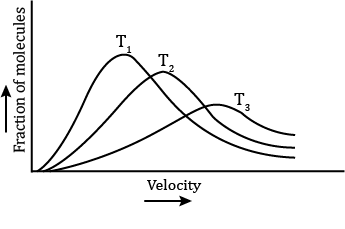
\includegraphics[height=.25\textheight]{res/maxwell.png}
  \captionsetup{justification=centering,margin=3cm}
  \caption{Phân bố Maxwell, được dùng trong động học chất khí để mô tả vận tốc
  các phân tử khí.}
\end{figure}
\end{frame}

\begin{frame}{Mô hình hóa quần thể bằng lý thuyết xác suất}
  Ta có một số các giả định như sau:
  \begin{itemize}
  \item Khi khởi tạo quần thể, ta thu được một phân bố quần thể là một phân bố
    liên tục và luôn dương.
  \end{itemize}

  Khi quần thể của ta là vô cùng lớn, ta có thể coi quần thể là một phân bố xác
  suất. Các cá thể có nhiều cá thể giống mình sẽ tương ứng với các giá trị mà tại đó
  hàm mật độ xác suất (PDF) có giá trị lớn và ngược lại.

  Tại thế hệ thứ \( g \),ta chia quần thể chung \( P^{g} \) với PDF \( p^{g}(x)
  \) thành các quần thể con \( P_{k}^{g} \), gồm có các cá thể có loài \( k \)
  (skill factor là \( k \)). Quần thể con \( P^{g}_{k} \) có hàm mật độ xác suất
  \( p^{g}_{k}(x) \):
\[
  p^{g}(x) = w_{1}p^{g}_{1}(x) + 
w_{2}p^{g}_{2}(x) + 
\ldots +
w_{T}p^{g}_{T}(x)
,\]
với các trọng số \( w_{i} \) là tỉ lệ số loài của quần thể con trong quần thể
chung: \( w_{k} = \frac{|P_{k}|}{|P|} \).
\end{frame}

\begin{frame}{Mô hình hóa quần thể bằng lý thuyết xác suất}
  Bali \textit{et al.} chứng minh được công thức sau, cho biết PDF của quần thể
  gồm các cá thể con loài \( k \) được sinh ra cũng là một tổ hợp tuyến tính của
  các hàm \( p_{1}^{g}, p_{2}^{g}, \ldots, p_{T}^{g} \):
  \begin{align*}
    q^{g}_{k}(x) &= \sum_{i = 1}^{T} \alpha_{i}^{g} p_{i}^{g}(x)\\
    \alpha_{k} &= 1- \frac{(T-1)rmp}{2T}\\
    \alpha_{j} &= \frac{rmp}{2T}, \forall j \neq  k\\
  .\end{align*}
\end{frame}
\begin{frame}{Mô hình hóa quần thể bằng lý thuyết xác suất}
  Quá trình chọn lọc cũng có thể được mô hình bằng công thức sau:
  \[
    p^{g+1}_{k}(x) = \begin{cases}
      \frac{q^{g}_{k}(x)}{\theta }, &\text{ nếu }f_{k}(x) \ge \beta^{g}_{k}\\
      0, & \text{ nếu ngược lại}
    \end{cases}
  ,\] 
  với \( \beta^{g}_{k} \) là ngưỡng chọn lọc của bài toán \( k \) trong thế hệ
  \( g \), \( \theta \) là tỷ lệ các cá thể được chọn:
  \[
    \int _{f_{k}(x) \ge \beta^{g}_{k}} q^{g}_{k}(x) = \theta
  .\] 
\end{frame}
\begin{frame}{Mô hình hóa quần thể bằng lý thuyết xác suất}
  Mặt khác, ta lại có:
  \begin{align*}
    \theta = \int _{f_{k}(x) \ge \beta^{g+1}_{k}} q^{g+1}_{k}(x)dx &= \alpha_{k}\int
    _{f_{k}(x) \ge \beta^{g+1}_{k}} p^{g+1}_{k}(x)dx + \underbrace{\sum_{\substack{i = 1\\i \neq    k}}^{T}\alpha_{i}\int
  _{f_{k}(x) \ge \beta^{g+1}_{k}} p^{g+1}_{i}(x)}_{\ge 0} \\
&\ge \alpha_{k} \int_{f_{k}(x) \ge B} p^{g+1}_{k}(x)dx, (B = \max
  \{\beta^{g}_{k}, \beta^{g+1}_{k}\}  )
  .\end{align*}

  Nếu \( \alpha_{k} > \theta \), thì tích phân cuối phải nhỏ hơn \( 1 \). Mà
  do \( \int _{f_{k}(x) \ge \beta^{g+1}_{k}} p^{g+1}_{k}(x) = 1 \) nên bắt buộc
  \( B < \beta^{g+1}_{k} \iff \boxed{\beta^{g}_{k} < \beta^{g+1}_{k}} \)
\end{frame}

\begin{frame}{Mô hình hóa quần thể bằng lý thuyết xác suất}
  Do \( \beta^{g}_{k} \) tăng (theo \( g \)) nên dãy này hội tụ tại \( f'_{k}
  \). Nếu giới hạn này lớn hơn giá trị tối ưu của hàm \( f_{k} \), ta có thể
  chứng minh sự mâu thuẫn bằng cách sử dụng đánh giá sau:
  \[
    p^{g}_{k}(x) \ge \left( \frac{\alpha_{k}}{\theta} \right) ^{g} p^{0}_{k}(x),
    \forall x: f_{k}(x) > f'_{k}
  ,\] suy được từ đánh giá tích phân.

  Do đó, cho \( g \to +\infty \), hàm \( p_{k} \) hội tụ đến vô cùng trên một
  đoạn có độ đo khác \( 0 \) (tập \( H \) gồm các điểm \( x \) thỏa mãn \(
  f_{k}(x) > f'_{k}\)), nên ta có:
  \[
    \lim_{g \to \infty} \int_{H} p^{g}_{k}(x) = +\infty
  .\] 
  Giới hạn này mâu thuẫn với việc các hàm \( p^{g}_{k} \) là các hàm mật độ xác
  suất. Do đó, \( \beta^{g}_{k} \) hội tụ tới giá trị tối ưu của hàm \(
  f_{k} \), nên thuật toán luôn luôn hội tụ cho bài toán \( k \) nếu có điều
  kiện \( \alpha_{k} > \theta \).
\end{frame}
\begin{frame}{Mô hình hóa quần thể bằng lý thuyết xác suất}
  Mặt khác, do \( \alpha_{k} = 1 - \frac{(T-1)rmp}{2T} > \frac{1}{2} \), nên
  thuật toán luôn luôn hội tụ (theo lý thuyết) nếu trong bước chọn lọc ta chỉ
  giữ lấy ít hơn một nửa số cá thể.

  Hơn nữa, từ những đánh giá trên, Bali \textit{et al.} còn đánh giá được
  rằng tốc độ hội tụ của thuật toán càng nhanh nếu phân phối \( q^{g}_{k} \)
  càng giống với \( p^{g}_{k} \). Do đó, theo đánh giá này, nếu \( rmp = 0
  \), \( \alpha_{k} = 1 \) và \( \alpha_{j} = 0 \) với mọi \( j \neq k \), thì
  \( p^{g}_{k} = q^{g}_{k} \) và theo lý thuyết thuật toán sẽ hội tụ nhanh nhất.
\end{frame}
% subsection Khảo sát tính hội tụ của thuật toán MFEA (end)

\subsection{Điều chỉnh xác suất lai ghép khác loài} % (fold)
\label{sub:Điều chỉnh xác suất lai ghép khác loài}

\begin{frame}{Ma trận xác suất lai ghép}
Trong phần trước, ta thấy rằng \( rmp \) càng làm cho phân phối của quần thể con
giống với quần thể cha mẹ thì quá trình chuyển giao tri thức càng hiệu quả. Với
ý tưởng này, ta có thể thực hiện cập nhật ma trận xác suất lai ghép một cách tự
động.

Trước hết, ta chuyển từ sử dụng một số \( rmp \) sang sử dụng ma trận \( RMP \):
\[
  RMP = \begin{bmatrix}
    RMP_{1, 1} & RMP_{1, 2} & \ldots \\
    RMP_{2,1} & RMP_{2,2} & \ldots \\
    \vdots & \vdots & \ddots
  \end{bmatrix} 
.\]
Ở đây, \( RMP_{i,j} \) là xác suất lai ghép giữa loài \( i \) và loài \( j \).
Vì trong thuật toán gốc ta luôn cho phép lai ghép cùng loài, nên \( RMP_{i,i} =
1, \forall i=\overline{1,T}\).

Ta không làm như thế này ở thuật toán gốc là vì việc sử dụng một ma trận RMP như
thế này sẽ sinh ra quá nhiều tham số. Do những tham số này sẽ được cập nhật tự
động trong thuật toán này, sử dụng nhiều tham số không còn là một vấn đề nữa.
\end{frame}


\begin{frame}{Cập nhật xác suất lai ghép}
  Để đo lường sự tương đồng giữa hai phân phối của quần thể con (có hàm PDF là
  \( q_{k}^{g}(x) \)) và quần thể cha mẹ (có hàm PDF là \( p_{k}^{g}(x) \)), ta
  sử dụng độ phân kỳ Kullback-Leibler:
  \[
    KL(P^{g}_{k}\mid \mid Q^{g}_{k}) = \int_{X} p^{g}_{k}(x) \log
    \frac{p^{g}_{k}(x)}{q^{g}_{k}(x)} dx
  .\] 
  Trong đó, \( X \) là không gian bao gồm mọi cá thể hợp lệ của bài toán thứ \(
  k\).

  Giá trị này thường được coi là một độ đo giữa hai phân phối. Nó càng nhỏ nếu
  hai phân phối càng gần nhau và ngược lại. Do đó, ta sẽ cập nhật \( RMP \) để
  làm cho giá trị này đạt giá trị nhỏ nhất.
\end{frame}

\begin{frame}{Cập nhật xác suất lai ghép}
  Đầu tiên, ta thấy:
  \[
    KL(P^{g}_{k}\mid \mid Q^{g}_{k}) = \underbrace{\int_{X} p^{g}_{k}(x) \log
    p^{g}_{k}(x)dx}_{\text{const}} - \int_{X} p^{g}_{k}(x) \log q^{g}_{k}(x)dx
  .\] 

  Do đó, ta sẽ cần tối đa tích phân \( \int_{X} p^{g}_{k}(x) \log q^{g}_{k}(x)dx
  \). Tích phân này lại chính là kì vọng của biến ngẫu nhiên \( \log
  q^{g}_{k}(P^{g}_{k}) \).

  Sau khi rởi rạc hóa, ta đưa bài toán ban đầu thành:
  \[
    \max c_{k}(RMP) = \sum_{x \in P^{g}_{k}} \log q^{g}_{k}(x)
  .\]
\end{frame}

\begin{frame}{Cập nhật xác suất lai ghép}
  Do ta có \( T \) hàm mục tiêu cho bài toán tối ưu \( RMP \), nên ta cần đưa
  bài toán đa mục tiêu này về bài toán đơn mục tiêu:
  \[
    \max c(RMP) = \sum_{k = 1}^{T} c_{k}(RMP) = \sum_{k = 1}^{T} \sum_{x \in
    P^{g}_{k}} \log q^{g}_{k}(x)
  .\] 
  Công thức của hàm \( q^{g}_{k} \) được tính qua hàm \( p^{g}_{k} \). Hàm này
  sẽ được ước tính tử quần thể \( P^{g}_{k} \). Ngoài ra, công thức của các hệ
  số \( \alpha_{k} \) cũng thay đổi do biến \( RMP \) là một ma trận:
  \begin{gather*}
    \alpha_{j} = \frac{RMP_{k,j}}{2T}, \forall  j \neq k\\
    \alpha_{k} = 1 - \frac{1}{2T}\sum_{j \neq  k} RMP_{k, j}\\
    q^{g}_{k}(x) = \sum_{j = 1}^{T} \alpha_{j}p^{g}_{j}(x)
  .\end{gather*}
\end{frame}

\begin{frame}{Cập nhật xác suất lai ghép}
  Vậy, quá trình cập nhật ma trận xác suất lai ghép \( RMP \) có thể được tóm
  tắt bằng các bước sau:
  \begin{itemize}
  \item Ước lượng các quần thể con \( P^{g}_{k} \) bằng các phân phối liên tục có
    hàm mật độ là \( p^{g}_{k} \).
  \item Từ các hàm mật độ sự phân bố  các cá thể cha mẹ \( p^{g}_{k} \), tính
    hàm mật độ cho các cá thể con \( q^{g}_{k} \).
  \item Thay các hàm \( q^{g}_{k} \) vào bài toán tối ưu biến \( RMP \) và giải
    bài toán này.
  \end{itemize}

  Thuật toán MFEA có sử dụng thêm phương pháp cập nhật xác suất lai ghép này
  được gọi là thuật toán \textbf{MFEA-II}.
\end{frame}
% subsection Điều chỉnh xác suất lai ghép khác loài (end)

% section Thuật toán Tiến hóa Đa yếu tố (MFEA) (end)
